\documentclass[landscape]{article}

\usepackage[a4paper,margin=1.5cm]{geometry}
\usepackage{tikz}
\usetikzlibrary{trees,calc,shapes,arrows.meta,positioning}
\usepackage{xcolor}
\usepackage{caption}
\usepackage{amsmath,amssymb}

% Custom colors
\definecolor{rosita}{RGB}{255,20,147}
\definecolor{darkgreen}{RGB}{0,120,0}
\definecolor{darkblue}{RGB}{0,0,180}
\definecolor{darkred}{RGB}{200,0,30}

% Custom commands
\newcommand{\playerA}{\textcolor{darkgreen}{Player A}}
\newcommand{\playerB}{\textcolor{darkblue}{Player B}}
\newcommand{\Dominated}{\textcolor{darkred}{Dominated Strategies}}

\pagestyle{empty}
\begin{document}
\thispagestyle{empty} %Para no poner número de página 

\begin{figure}
	\centering
	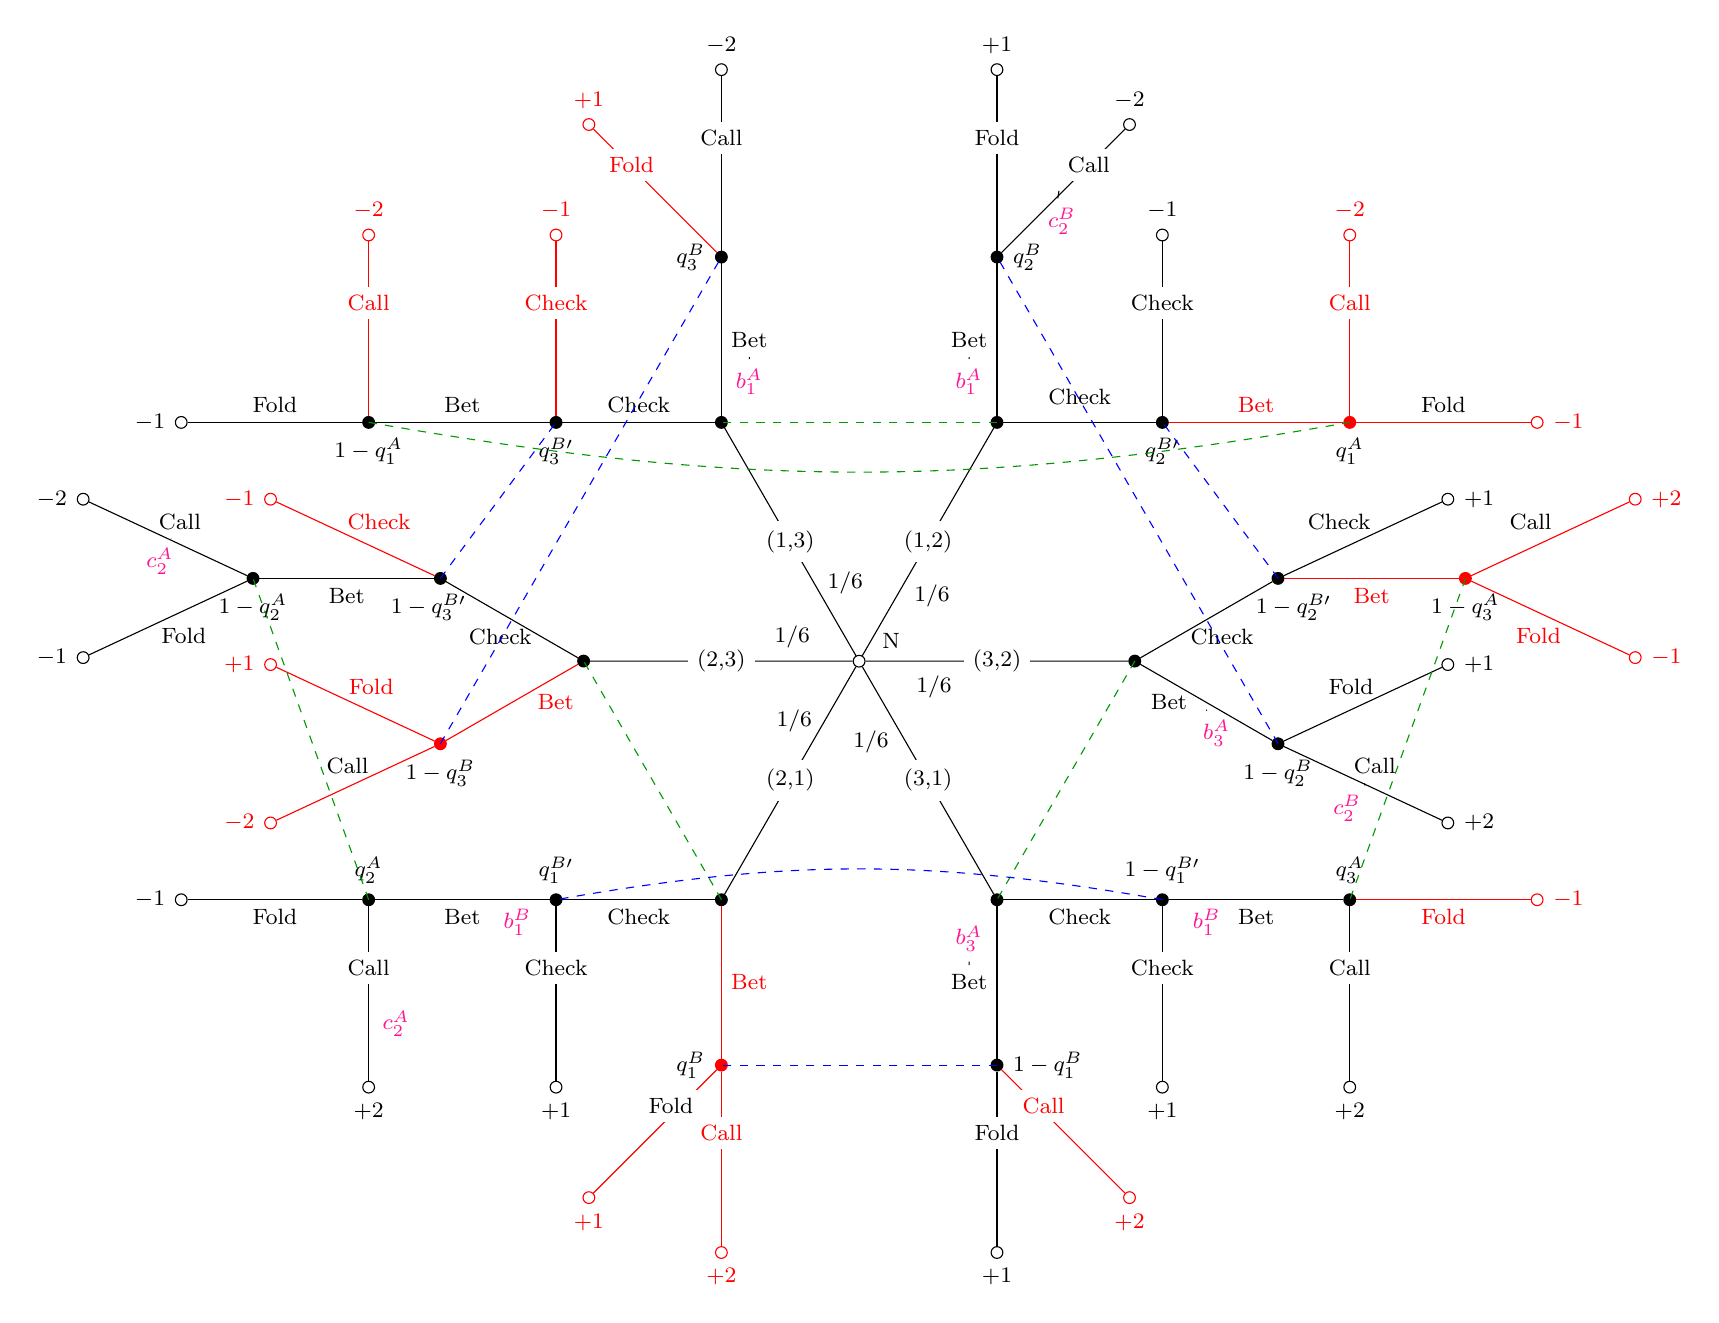
\begin{tikzpicture}
		[scale=1.4,font=\footnotesize,remember picture]
		\tikzset{
			% Two node styles for game trees: solid and solid
			solid node/.style={circle,draw,inner sep=1.5,fill=black},
			hollow node/.style={circle,draw,inner sep=1.5}
		}
		% Specify spacing for each level of the tree
		\tikzstyle{level 1}=[level distance=25mm,sibling distance=25mm]
		\tikzstyle{level 2}=[level distance=15mm,sibling distance=15mm]
		\tikzstyle{level 3}=[level distance=17mm,sibling distance=10mm]
		
		% The Tree
		\node(0)[hollow node,label=30:{\hspace{0.1cm}N}] at (current page.center) {} % Nodo raíz "N" en el centro
		% Nodo arriba a la derecha
		child[grow=60]{
			node(1)[solid node]{}
			child[grow=right]{node (12c)[solid node,label=-90:{$q_2^{B\prime}$}]{}
				child[grow=right, red]{node (12)[solid node,label=-90:{\textcolor{black}{$q_1^A$}}, red]{}
					child[grow=right]{node[hollow node,label=right:{$-1$}]{}  edge from parent node [above, black]{Fold}}
					child[grow=up]{node[hollow node,label=above:{$-2$}]{} edge from parent node [above]{\colorbox{white}{\textcolor{red}{Call}}}}
					edge from parent node [above]{\textcolor{red}{Bet}}}
				child[grow=up]{node[hollow node,label=above:{$-1$}]{} edge from parent node [above]{\colorbox{white}{Check}}}
				edge from parent node [above]{\colorbox{white}{Check}}}
			child[grow=up]{node(12b)[solid node,label=right:{$q_2^{B}$}]{}
				child[grow=90]{node[hollow node,label=above:{$+1$}]{} edge from parent node [above]{\colorbox{white}{Fold}}}
				child[grow=45]{node[hollow node,label=above:{$-2$}]{} edge from parent node [above]{\colorbox{white}{\hspace{0.55cm} Call}} child[grow=south, level distance=0mm]{node[anchor=68][yshift=-12pt]{\hspace{0.2cm}\textcolor{rosita}{$c_2^B$}}}}
				edge from parent node [left]{Bet}
				child[grow=down, level distance=0mm]{node[anchor=north][yshift=-7pt]{\textcolor{rosita}{$b_1^A$}}} 
			}
		} 
		% Nodo derecha
		child[grow=right]{
			node(2)[solid node]{}
			child[grow=30]{node(32c)[solid node,label=-90:{\hspace{0.3cm} $1-q_2^{B\prime}$}]{}
				child[grow=right, red]{node (32)[solid node,label=-90:{\textcolor{black}{$1-q_3^A$}}, red]{}
					child[grow=-25]{node[hollow node,label=right:{$-1$}]{}  edge from parent node [below]{\textcolor{red}{\hspace{-0.3cm}Fold}}}
					child[grow=25]{node[hollow node,label=right:{$+2$}]{} edge from parent node [above, black]{\hspace{-0.5cm}Call}}
					edge from parent node [below]{\textcolor{red}{Bet}}}
				child[grow=25]{node[hollow node,label=right:{$+1$}]{} edge from parent node [above]{\hspace{-0.6cm}Check}}
				edge from parent node [below]{\hspace{0.3cm} Check}}
			child[grow=-30]{node(32b)[solid node,label=-90:{$1-q_2^{B}$}]{}
				child[grow=25]{node[hollow node,label=right:{$+1$}]{} edge from parent node [above]{\hspace{-0.4cm} Fold}}
				child[grow=-25]{node[hollow node,label=right:{$+2$}]{} edge from parent node [above]{{\hspace{0.2cm} Call}} child[grow=south, level distance=0mm]{node[anchor=170][yshift=-15pt]{\hspace{-0.5cm}\textcolor{rosita}{$c_2^B$}}}}
				edge from parent node [left]{\hspace{-0.9cm}Bet}
				child[grow=right, level distance=0mm]{node[anchor=110][yshift=-3pt] {\hspace{0cm} \textcolor{rosita}{$b_3^A$}}}
			}
		}
		% Nodo arriba izquierda
		child[grow=120]{
			node(6)[solid node]{}
			child[grow=left]{node (13b)[solid node,label=-90:{$q_3^{B\prime}$}]{}
				child[grow=left]{node(13)[solid node,label=-90:{$1-q^{A}_1$}]{}
					child[grow=left]{node[hollow node,label=left:{$-1$}]{}  edge from parent node [above]{Fold}}
					child[grow=up, red]{node[hollow node,label=above:{$-2$}]{} edge from parent node [above]{\colorbox{white}{\textcolor{red}{Call}}}}
					edge from parent node [above]{Bet}}
				child[grow=up, red]{node[hollow node,label=above:{$-1$}]{} edge from parent node [above]{\colorbox{white}{\textcolor{red}{Check}}}}
				edge from parent node [above]{Check}}
			child[grow=up]{node(13c)[solid node,label=left:{$q_3^{B}$}]{}
				child[grow=90]{node[hollow node,label=above:{$-2$}]{} edge from parent node [above]{\colorbox{white}{Call}
				}}
				child[grow=-225, red]{node[hollow node,label=above:{$+1$}]{} edge from parent node [above]{\hspace{-0.6cm}\colorbox{white}{\textcolor{red}{Fold}}}}
				edge from parent node [right]{Bet}
				child[grow=down, level distance=0mm]{node[anchor=north][yshift=-7pt]{\textcolor{rosita}{$b_1^A$}}} 
			}
		}
		% Nodo abajo derecha
		child[grow=-60]{
			node(3)[solid node]{}
			child[grow=right]{node(1bp)[solid node,label=:{$1-q_1^{B\prime}$}]{}
				child[grow=right]{node(31)[solid node,label=90:{$q_3^A$}]{}
					child[grow=right, red]{node[hollow node,label=right:{$-1$}]{}  edge from parent node [below]{\textcolor{red}{Fold}}}
					child[grow=down]{node[hollow node,label=below:{$+2$}]{} edge from parent node [above]{\colorbox{white}{Call}}}
					edge from parent node [below]{{Bet}} child[grow=north, level distance=0mm]{node[anchor=180][yshift=-2pt]{\hspace{-1.3cm}\textcolor{rosita}{$b_1^B$}}}}
				child[grow=down]{node[hollow node,label=below:{$+1$}]{} edge from parent node [above]{ \colorbox{white}{Check}}}
				edge from parent node [below]{Check}}
			child[grow=down]{node(1b)[solid node,label=right:{$1-q_1^{B}$}]{}
				child[grow=-90]{node[hollow node,label=below:{$+1$}]{} edge from parent node [above]{\colorbox{white}{Fold}}}
				child[grow=-45, red]{node[hollow node,label=below:{$+2$}]{} edge from parent node [above]{\hspace{-0.5cm}\colorbox{white}{\textcolor{red}{Call}}}}
				edge from parent node [left]{Bet}
				child[grow=up, level distance=0mm]{node[anchor=north][yshift=24pt]{\textcolor{rosita}{$b_3^A$}}} 
			}
		}
		% Nodo izquierda
		child[grow=left]{
			node(5)[solid node]{}
			child[grow=150]{node (23b)[solid node,label=-90:{\hspace{-0.3cm}$1-q_3^{B\prime}$}]{}
				child[grow=left]{node (23)[solid node,label=-90:{$1-q_2^A$}]{}
					child[grow=205]{node[hollow node,label=left:{$-1$}]{}  edge from parent node [below]{\hspace{0.4cm}Fold}}
					child[grow=155]{node[hollow node,label=left:{$-2$}]{} edge from parent node [above]{\hspace{0.2cm} Call} child[grow=south, level distance=0mm]{node[anchor=170][yshift=-14pt]{\hspace{-0.4cm}\textcolor{rosita}{$c_2^A$}}}}     
					edge from parent node [below]{Bet}}
				child[grow=155, red]{node[hollow node,label=left:{$-1$}]{} edge from parent node [above]{\textcolor{red}{\hspace{0.5cm} Check}}}
				edge from parent node [below]{\hspace{-0.4cm} Check}}
			child[grow=210, red]{node (23c)[solid node,label=-90:{\textcolor{black}{$1-q_3^{B}$}}, red]{}
				child[grow=155]{node[hollow node,label=left:{$+1$}]{} edge from parent node [above]{\textcolor{red}{\hspace{0.3cm} Fold}}}
				child[grow=205]{node[hollow node,label=left:{$-2$}]{} edge from parent node [above, black]{\hspace{-0.2cm}Call}}
				edge from parent node [right]{\textcolor{red}{\hspace{0.2cm}Bet}}
			}
		}
		% Nodo abajo izquierda
		child[grow=-120]{
			node(4)[solid node]{}
			child[grow=left]{node(bp)[solid node,label=:{$q_1^{B\prime}$}]{}
				child[grow=left]{node(21)[solid node,label=90:{$q_2^A$}]{}
					child[grow=left]{node[hollow node,label=left:{$-1$}]{}  edge from parent node [below]{Fold}}
					child[grow=down]{node[hollow node,label=below:{$+2$}]{} edge from parent node [above]{\colorbox{white}{Call}} child[grow=south, level distance=0mm]{node[anchor=north][yshift=-12pt]{\hspace{0.7cm}\textcolor{rosita}{$c_2^A$}}}}
					edge from parent node [below]{{Bet}} child[grow=north, level distance=0mm]{node[anchor=180][yshift=-2pt]{\hspace{0.4cm}\textcolor{rosita}{$b_1^B$}}}}
				child[grow=down]{node[hollow node,label=below:{$+1$}]{} edge from parent node [above]{\colorbox{white}{Check}}}
				edge from parent node [below]{Check}}
			child[grow=down, red]{node(b)[solid node,label=left:{\textcolor{black}{$q_1^{B}$}}, red]{}
				child[grow=-90]{node[hollow node,label=below:{$+2$}, red]{} edge from parent node [above]{\colorbox{white}{\textcolor{red}{Call}}}}
				child[grow=225]{node[hollow node,label=below:{$+1$}]{} edge from parent node [above, black]{\hspace{0.4cm}{\colorbox{white}{Fold}}}}
				edge from parent node [right]{\textcolor{red}{Bet}}
			}
		};
		
		% Information sets para A, en rojo
		\draw[dashed,rounded corners=1, green!60!black]($(1)$)to[fill=white] ($(6)$);
		\draw[dashed,rounded corners=10,green!60!black]($(2)$)to[fill=white]($(3)$);
		\draw[dashed,rounded corners=10,green!60!black]($(4)$)to[fill=white]($(5)$);
		\draw[dashed,rounded corners=10,green!60!black]($(21)$)--($(23)$);
		\draw[dashed,rounded corners=10,green!60!black]($(13)$)to[bend right=10]($(12)$);
		\draw[dashed,rounded corners=10,green!60!black]($(32)$)--($(31)$);
		
		% Information sets para B, en azul
		\draw[dashed,rounded corners=10,blue]($(1b)$)to[fill=white]($(b)$);
		\draw[dashed,rounded corners=10,blue]($(1bp)$)to[bend right=10]($(bp)$);
		\draw[dashed,rounded corners=10,blue]($(23b)$)to[fill=white]($(13b)$);
		\draw[dashed,rounded corners=10,blue]($(23c)$)to[fill=white]($(13c)$);
		\draw[dashed,rounded corners=10,blue]($(32c)$)to[fill=white]($(12c)$);
		\draw[dashed,rounded corners=10,blue]($(32b)$)to[fill=white]($(12b)$);
		
		% Definimos nodos para agregar probabilidades y cartas
		\node at ($(1b)!.5!(b)$)[] {};
		\node at ($(1bp)!.5!(bp)$)[] {};
		\node at ($(1)!.5!(6)$) []{};
		\node at ($(2)!.5!(3)$) []{};
		\node at ($(4)!.5!(5)$)[] {};
		\node at ($(23b)!.5!(13b)$)[] {};
		\node at ($(23c)!.5!(13c)$)[] {};
		\node at ($(32c)!.5!(12c)$)[] {};
		\node at ($(32b)!.5!(12b)$)[] {};
		\node at ($(21)!.5!(23)$)[] {};
		\node at ($(13)!.5!(12)$)[] {};
		\node at ($(32)!.5!(31)$)[] {};
		\node at ($(6)!.5!(0)$) [fill=white] {(1,3)};
		\node at ($(6)!.5!(0)$) [right, yshift=-15pt] {\hspace{0.25cm} 1/6};
		\node at ($(5)!.5!(0)$) [fill=white]{(2,3)};
		\node at ($(5)!.5!(0)$) [above, yshift=1pt]{\hspace{1.7cm} 1/6};
		\node at ($(4)!.5!(0)$)[fill=white] {(2,1)};
		\node at ($(4)!.5!(0)$) [above, yshift=14pt] {\hspace{0cm} 1/6};
		\node at ($(3)!.5!(0)$) [fill=white]{(3,1)};
		\node at ($(3)!.5!(0)$) [left, yshift=14pt] {\hspace{-1.5cm} 1/6};
		\node at ($(2)!.5!(0)$)[fill=white] {(3,2)};
		\node at ($(2)!.5!(0)$) [below, yshift=-2pt]{\hspace{-1.7cm} 1/6};
		\node at ($(1)!.5!(0)$)[fill=white] {(1,2)};
		\node at ($(1)!.5!(0)$) [below, yshift=-12pt] {\hspace{0cm} 1/6};
		
	\end{tikzpicture}
	\captionsetup{skip=1cm} % Move the caption below
	\caption[Kuhn Poker]{Kuhn Poker \text{\playerA}\hspace{0.5em}\text{\playerB}\hspace{0.5em}\text{\Dominated}\hspace{0.5em}} % Caption of the figure
	\label{fig:figure}
\end{figure}

\end{document}
